% Chapter 9 -- English manuscript fragment.
% Required packages in the parent manuscript: amsmath, amssymb, booktabs,
% graphicx, array, and xcolor.

\section{Numerical Evaluation}
\label{sec:numerical_evaluation}

\subsection{Objective and protocol overview}
\label{sec:evaluation_objective}

The experiment evaluates whether the proposed smooth-to-hard spectral regularizer improves dynamic cardiac MR reconstruction relative to singular-value Soft thresholding, discontinuous Hard thresholding, and low-rank plus sparse (L+S) reconstruction over a prespecified range of accelerations and measurement-noise levels. The same formal OCMR series, sampling masks, noisy measurements, validation splits, and stopping rule were used for all four methods. All retrospective degradation was applied after coil compression, frame-wise sensitivity estimation, and sensitivity-weighted coil combination; hence, the reconstruction problem was a single-image Cartesian inverse problem (Fig.~\ref{fig:evaluation_pipeline}).

\begin{figure*}[t]
  \centering
  \begingroup
  \setlength{\tabcolsep}{2pt}
  \renewcommand{\arraystretch}{1.12}
  \newcommand{\pipebox}[1]{\fbox{\parbox[c][1.05cm][c]{0.205\textwidth}{\centering\small #1}}}
  \resizebox{\textwidth}{!}{%
  \begin{tabular}{c@{\;${\longrightarrow}$\;}c@{\;${\longrightarrow}$\;}c@{\;${\longrightarrow}$\;}c}
    \pipebox{Fully sampled multi-coil cine} &
    \pipebox{POCS if required; compression to 12 virtual coils} &
    \pipebox{Frame-wise ESPIRiT sensitivity maps} &
    \pipebox{Sensitivity-weighted coil combination} \\
    \multicolumn{4}{c}{$\Downarrow$} \\
    \pipebox{RMS-normalized complex reference} &
    \pipebox{Single-image Fourier sampling and complex noise} &
    \pipebox{Training/validation split and candidate selection} &
    \pipebox{Full-data refit and paired evaluation}
  \end{tabular}}
  \endgroup
  \caption{Evaluation pipeline. Coil processing was completed before retrospective undersampling and noise addition; every method therefore received the same noisy, undersampled single-image $k$-space data.}
  \label{fig:evaluation_pipeline}
\end{figure*}

\subsection{Data and single-image preprocessing}
\label{sec:data_preprocessing}

Fully sampled multi-coil cardiac cine data were obtained from OCMR~[2]. Four series were reserved for pipeline checks, candidate construction, and parameter-boundary auditing. The disjoint formal cohort contained 20 series: 10 short-axis and 10 long-axis acquisitions, nine acquired at 1.5~T and eleven at 3~T, with 16--27 cardiac phases (median 21.5). Because public patient identifiers were unavailable, the series were treated as the statistical units.

Readout oversampling was removed and each series was brought to its reconstruction matrix. Four formal series contained partial-Fourier readout; their missing samples were completed by eight fixed POCS iterations. A global semi-unitary compression basis then reduced the original 15--38 receiver coils to 12 virtual coils, retaining 97.68--99.29\% of the coil energy (median 98.69\%).

ESPIRiT sensitivity maps were estimated independently for each cardiac frame from the fully sampled virtual-coil data, using the full readout extent, 24 central $k_y$ calibration lines, a $6\times6$ kernel, a relative calibration singular-value threshold of $0.02$, and an image-domain eigenvalue threshold of zero. The combined reference frame was
\begin{equation}
  x_{0,t}=\sum_{c=1}^{12}\overline{\widehat S_{t,c}}\,
  \mathcal F^{-1}_{xy}k_{t,c},
  \label{eq:coil_combination}
\end{equation}
where $\widehat S_{t,c}$ and $k_{t,c}$ are the sensitivity map and fully sampled $k$-space of virtual coil $c$. The resulting complex cine $X_0$ was normalized by its root-mean-square amplitude,
\begin{equation}
  X_0\leftarrow X_0\bigg/
  \frac{\lVert X_0\rVert_F}{\sqrt{N_xN_yT}}.
  \label{eq:rms_normalization}
\end{equation}

\subsection{Retrospective acquisition model}
\label{sec:acquisition_model}

After coil combination, the forward operator was
\begin{equation}
  \mathcal A_{\Omega}(X)=P_{\Omega}\mathcal F_{xy}X,
  \label{eq:single_image_forward}
\end{equation}
where $\mathcal F_{xy}$ is the orthonormal two-dimensional Fourier transform applied frame by frame. Acceleration factors were $R\in\{4,6,8\}$. Each frame retained $\operatorname{round}(N_y/R)$ phase-encoding lines, including eight central ACS lines. Peripheral lines followed a centre-weighted variable-density distribution with usage-dependent complementary temporal coverage; every selected line contained the complete readout direction.

Circular complex Gaussian noise was added to the acquired single-image $k$-space. With $s_{\Omega}=\mathcal A_{\Omega}(X_0)$, $m$ acquired complex samples, and $z=(z_{\mathrm r}+\mathrm i z_{\mathrm i})/\sqrt2$ for independent standard-normal $z_{\mathrm r}$ and $z_{\mathrm i}$,
\begin{equation}
  y_{\Omega}=s_{\Omega}+\sigma_qP_{\Omega}z,
  \qquad
  \sigma_q=\frac{\lVert s_{\Omega}\rVert_2}
  {\sqrt m\,10^{q/20}},
  \qquad q=\mathrm{SNR}_{\mathrm{nom}}.
  \label{eq:noise_scale}
\end{equation}
Thus, $q\in\{0,10,20,30\}$~dB is an input to the noise-scaling formula, not the noise amplitude itself: 0~dB produces the strongest noise and 30~dB the weakest. For each series and $R$, the same standard noise draw was rescaled across the four values of $q$. Realized measurement SNR differed from the nominal value by at most approximately 0.04~dB.

Table~\ref{tab:experimental_settings} summarizes the fixed protocol. Deterministic child seeds derived from the series identifier, acceleration, and purpose were generated from base seeds 2026100301 (masks), 2026100302 (validation), and 2026100303 (noise).

\begin{table*}[t]
\centering
\caption{Fixed experimental settings. Candidate sets were constructed with the four pilot series and frozen before evaluation of the 20 formal series.}
\label{tab:experimental_settings}
\small
\renewcommand{\arraystretch}{1.08}
\begin{tabular}{p{0.23\textwidth}p{0.70\textwidth}}
\toprule
Component & Setting \\
\midrule
Formal data & 20 OCMR series; 10 short-axis/10 long-axis; nine 1.5-T/eleven 3-T; 16--27 phases. \\
Pilot data & Four disjoint series used only for pipeline checks, candidate construction, and boundary auditing. \\
Partial Fourier & Eight POCS iterations for four formal series before coil compression. \\
Coil processing & Global compression to 12 virtual coils; frame-wise ESPIRiT with 24 central $k_y$ lines, $6\times6$ kernel, calibration threshold $0.02$, image eigenvalue threshold $0$; Eq.~\eqref{eq:coil_combination}; complex RMS normalization. \\
Sampling & $R\in\{4,6,8\}$; time-varying variable-density Cartesian masks; eight central ACS lines in every frame and included in the reported acceleration. \\
Noise & Eq.~\eqref{eq:noise_scale}; $q\in\{0,10,20,30\}$~dB; common standard draw across $q$ for fixed series and $R$. \\
Validation & 15\% of acquired peripheral line--time pairs; same split for all methods; ACS always retained in training. \\
Frozen candidates & Separate set for every method and $R\times q$ condition: six Proposed, four Soft, four Hard, and six L+S candidates. \\
Optimization & Relative iterate tolerance $10^{-5}$ or 300 iterations; Proposed scalar proximal-root tolerance $10^{-9}$. \\
Statistics & Paired series-level differences; mean, standard deviation, median, wins, and 95\% bootstrap interval of the mean from 20,000 paired resamples. \\
Metrics & Primary: magnitude PSNR. Complementary: complex NMSE and magnitude SSIM within the reference-defined ROI. \\
\bottomrule
\end{tabular}
\end{table*}

\subsection{Condition-specific parameter selection}
\label{sec:parameter_selection}

Candidate sets were allowed to differ by method, acceleration, and nominal SNR, but their construction used only the four pilot series. For each formal series and condition, 15\% of acquired peripheral line--time pairs formed a validation set; ACS samples remained in training. All methods used the same split. A candidate $\theta$ was fitted only to the training data and scored by
\begin{equation}
  V(\theta)=\frac{1}{m_{\mathrm{val}}}
  \left\lVert\mathcal A_{\mathrm{val}}(\widehat X_\theta)
  -y_{\mathrm{val}}\right\rVert_2^2.
  \label{eq:validation_score}
\end{equation}
The lowest-score candidate was selected independently for each series and condition and then refitted to all acquired samples. Reference-image metrics were not used for selection.

For Proposed, $\theta=(\alpha,a,c)$ and $\lambda=c\sigma_1(X_{\mathrm{init}})$. Soft and Hard used normalized thresholds $\tau=q_s\sigma_1(X_{\mathrm{init}})$. L+S used pairs $(q_L,q_S)$ with $\tau_L=q_L\sigma_1(X_{\mathrm{init}})$ and $\tau_S=q_S\max|\mathcal F_tX_{\mathrm{init}}|$. The retained sets were sparse collections of pilot-supported candidates rather than complete Cartesian products. This keeps the search computationally tractable while defining a fixed, condition-specific selection procedure for every method.

\subsection{Outcome measures and paired analysis}
\label{sec:evaluation_metrics}

Magnitude PSNR was the primary summary measure. Complex NMSE and magnitude SSIM were complementary measures used to assess whether the PSNR conclusions were consistent across error magnitude and structural fidelity. SSIM was averaged frame-wise inside a reference-defined ROI whose temporal-mean magnitude exceeded 5\% of its maximum.

All comparisons were paired by series and oriented so that positive values favoured Proposed:
\begin{equation}
  \Delta\mathrm{NMSE}_B=\mathrm{NMSE}_B-\mathrm{NMSE}_{\mathrm{P}},
  \quad
  \Delta\mathrm{PSNR}_B=\mathrm{PSNR}_{\mathrm{P}}-\mathrm{PSNR}_B,
  \quad
  \Delta\mathrm{SSIM}_B=\mathrm{SSIM}_{\mathrm{P}}-\mathrm{SSIM}_B.
  \label{eq:paired_differences}
\end{equation}
Condition-level summaries report the mean difference and number of positive differences; case-level distributions and 95\% nonparametric bootstrap intervals from 20,000 paired resamples are shown graphically. The intervals are descriptive and are not multiplicity-adjusted hypothesis tests.

\subsection{Reconstruction results}
\label{sec:evaluation_results}

Table~\ref{tab:single_image_psnr} gives the Proposed mean PSNR and its paired mean differences from each baseline. Proposed exceeded Hard in 11 of 12 conditions. The exception was $R=4$, 10~dB, where the mean difference was $-0.272$~dB (7/20 wins; 95\% bootstrap interval $[-0.506,-0.027]$~dB). Against Soft, Proposed was generally less favourable at 0--10~dB, mixed at 20~dB, and favourable at every 30-dB condition. Against L+S, Proposed was lower throughout 10~dB, mixed at 0 and 20~dB, and higher at every 30-dB condition.

\begin{table}[t]
\centering
\caption{Mean magnitude PSNR of Proposed and mean paired PSNR differences in dB (Proposed minus baseline), with Proposed wins in parentheses. $\mathrm{SNR}_{\mathrm{nom}}$ is the parameter $q$ in Eq.~\eqref{eq:noise_scale}; larger values mean less added noise. Each row contains 20 paired series.}
\label{tab:single_image_psnr}
\small
\setlength{\tabcolsep}{3.2pt}
\begin{tabular}{cccccc}
\toprule
$R$ & $\mathrm{SNR}_{\mathrm{nom}}$ & Proposed & $\Delta$ Hard & $\Delta$ Soft & $\Delta$ L+S \\
 & (dB) & PSNR (dB) & & & \\
\midrule
4 & 0  & 22.601 & $+2.664$ (20/20) & $-0.904$ (8/20)  & $+1.157$ (13/20) \\
4 & 10 & 29.547 & $-0.272$ (7/20)  & $-0.435$ (4/20)  & $-1.123$ (0/20) \\
4 & 20 & 37.271 & $+1.074$ (18/20) & $-0.082$ (6/20)  & $-0.329$ (2/20) \\
4 & 30 & 41.454 & $+3.386$ (20/20) & $+0.702$ (20/20) & $+0.623$ (18/20) \\
6 & 0  & 21.998 & $+4.222$ (20/20) & $-2.312$ (0/20)  & $+0.244$ (17/20) \\
6 & 10 & 28.581 & $+1.409$ (20/20) & $-0.937$ (0/20)  & $-0.814$ (0/20) \\
6 & 20 & 35.265 & $+0.798$ (19/20) & $+0.243$ (15/20) & $+0.184$ (14/20) \\
6 & 30 & 38.673 & $+1.876$ (20/20) & $+0.930$ (20/20) & $+1.062$ (19/20) \\
8 & 0  & 21.046 & $+3.183$ (16/20) & $-2.499$ (1/20)  & $-0.711$ (11/20) \\
8 & 10 & 27.518 & $+1.445$ (20/20) & $-0.625$ (1/20)  & $-0.708$ (2/20) \\
8 & 20 & 33.670 & $+0.488$ (19/20) & $+0.683$ (19/20) & $+0.749$ (18/20) \\
8 & 30 & 36.395 & $+1.003$ (20/20) & $+1.328$ (20/20) & $+1.777$ (20/20) \\
\bottomrule
\end{tabular}
\end{table}

Figure~\ref{fig:paired_psnr_distributions} shows that the 0-dB differences are wider and more skewed than those at higher nominal SNR. In particular, at $R=8$, 0~dB versus L+S, the mean was $-0.711$~dB but the median was $+0.336$~dB and the bootstrap interval crossed zero. The 0-dB row should therefore be interpreted as an extreme-noise regime with substantial case-to-case variability, rather than forced into a monotone trend.

\begin{figure*}[t]
  \centering
  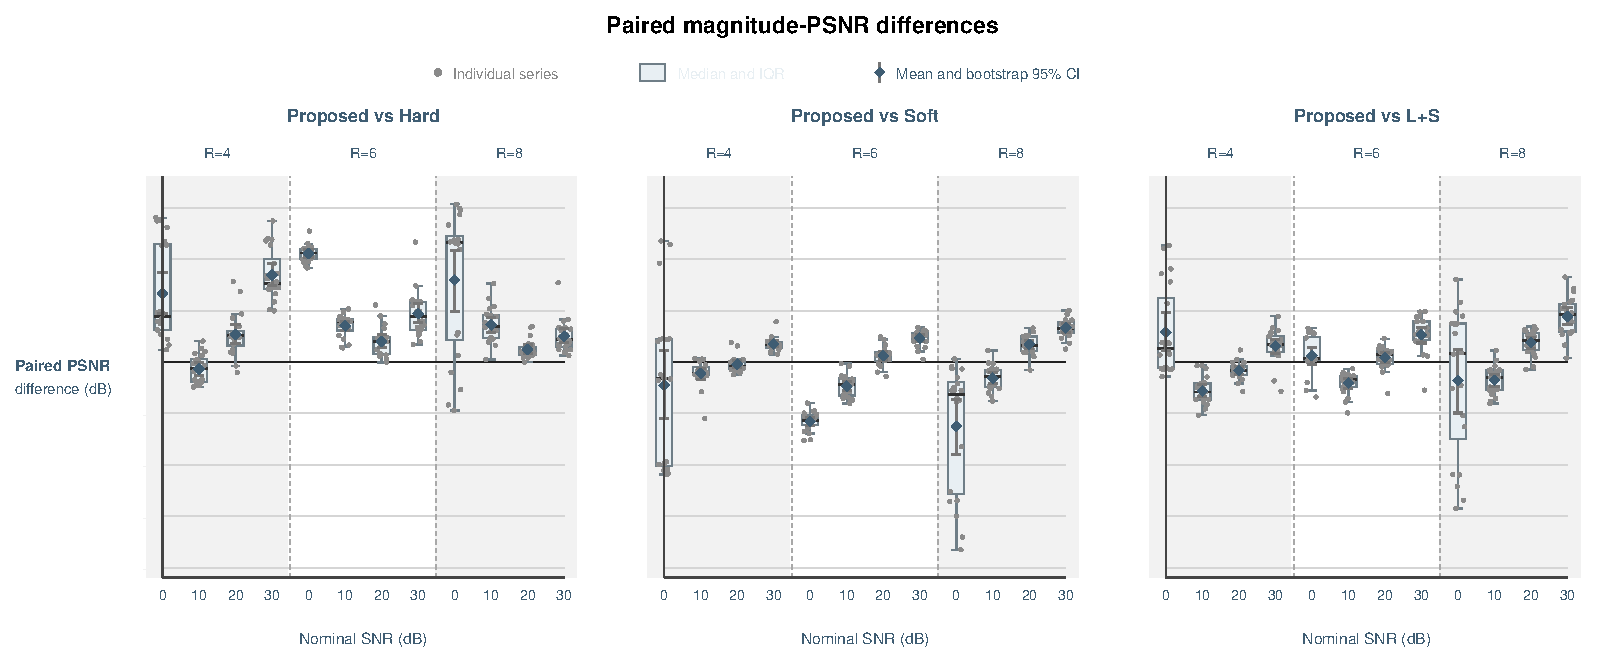
\includegraphics[width=\textwidth]{fig4_paired_psnr_distributions.pdf}
  \caption{Paired magnitude-PSNR differences for the 20 formal series. Positive values favour Proposed. Individual series, medians, interquartile ranges, means, and 95\% paired-bootstrap intervals show both the average effect and its case-level dispersion.}
  \label{fig:paired_psnr_distributions}
\end{figure*}

The complementary metrics in Fig.~\ref{fig:secondary_metrics} support the same condition-dependent interpretation. Relative to Hard, NMSE and SSIM were predominantly favourable or near neutral. Relative to Soft and L+S, their signs generally followed the PSNR crossover, while the widest intervals occurred under the strongest noise. These measures are supporting evidence rather than a second optimization target.

\begin{figure*}[t]
  \centering
  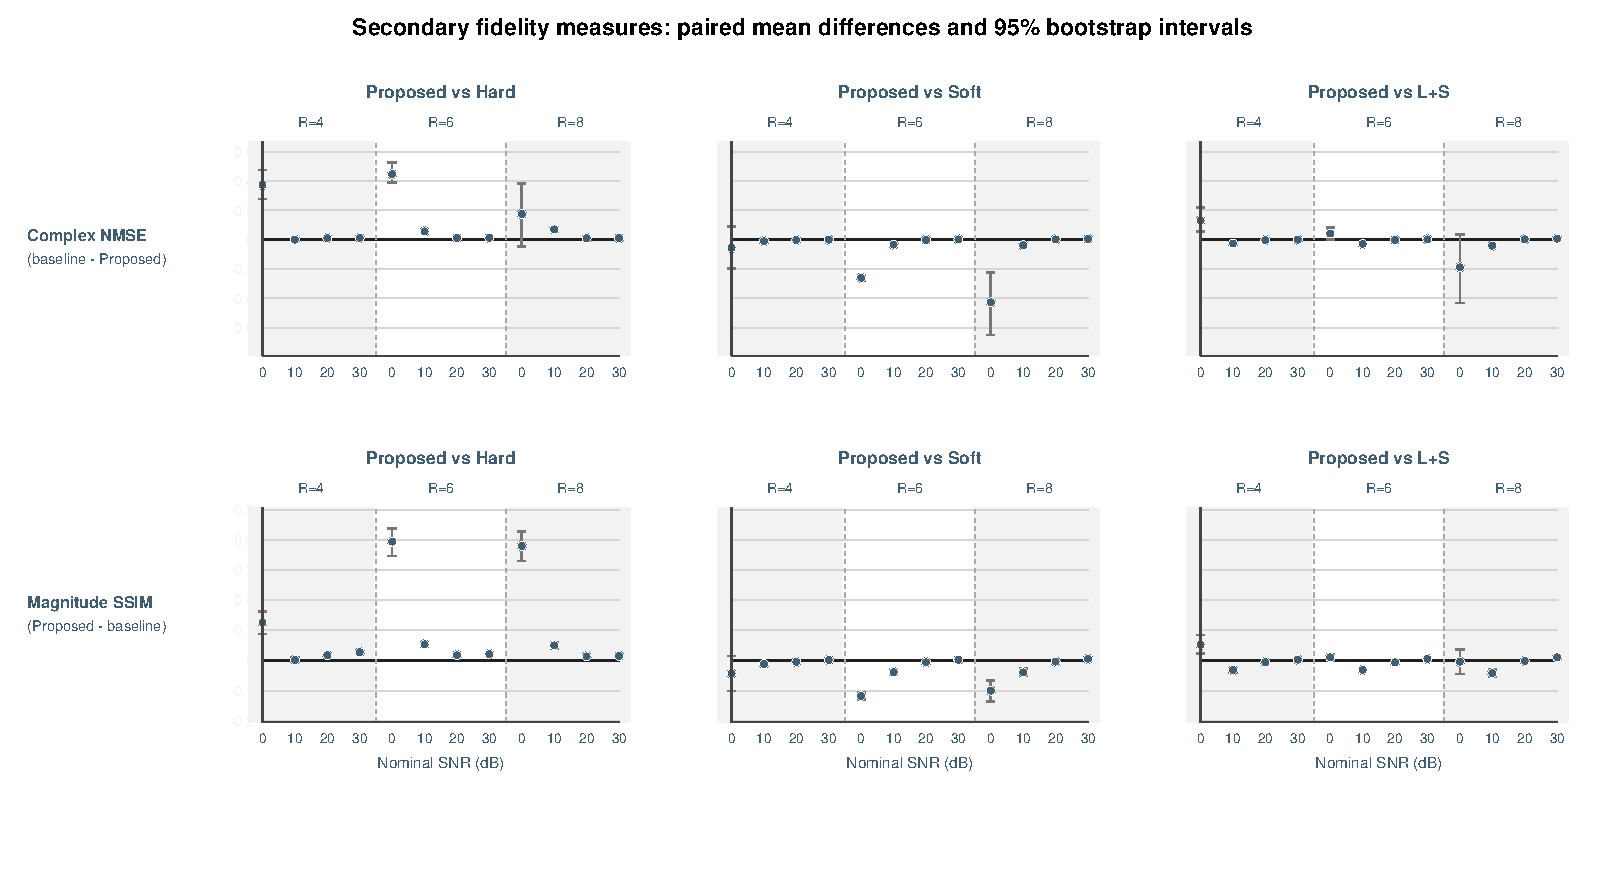
\includegraphics[width=\textwidth]{fig5_secondary_metric_intervals.pdf}
  \caption{Mean paired differences and 95\% paired-bootstrap intervals for complex NMSE and magnitude SSIM. NMSE is baseline minus Proposed; SSIM is Proposed minus baseline, so positive values favour Proposed in both rows. The restrained point-and-interval display replaces a metric-specific colour heatmap.}
  \label{fig:secondary_metrics}
\end{figure*}

Figure~\ref{fig:qualitative_temporal} presents two prespecified median-difference examples: Proposed versus Soft at $R=4$, 0~dB, and Proposed versus L+S at $R=8$, 30~dB. Each block contains the reference, the displayed-frame sampling mask, the noisy zero-filled reconstruction, all four reconstructions, and jet-coloured absolute-error maps. Error cells under the reference and mask are intentionally blank. The examples illustrate the severe-noise stability of Soft and the reduced clean-data bias of Proposed without treating two cases as population-level evidence.

\begin{figure*}[p]
  \centering
  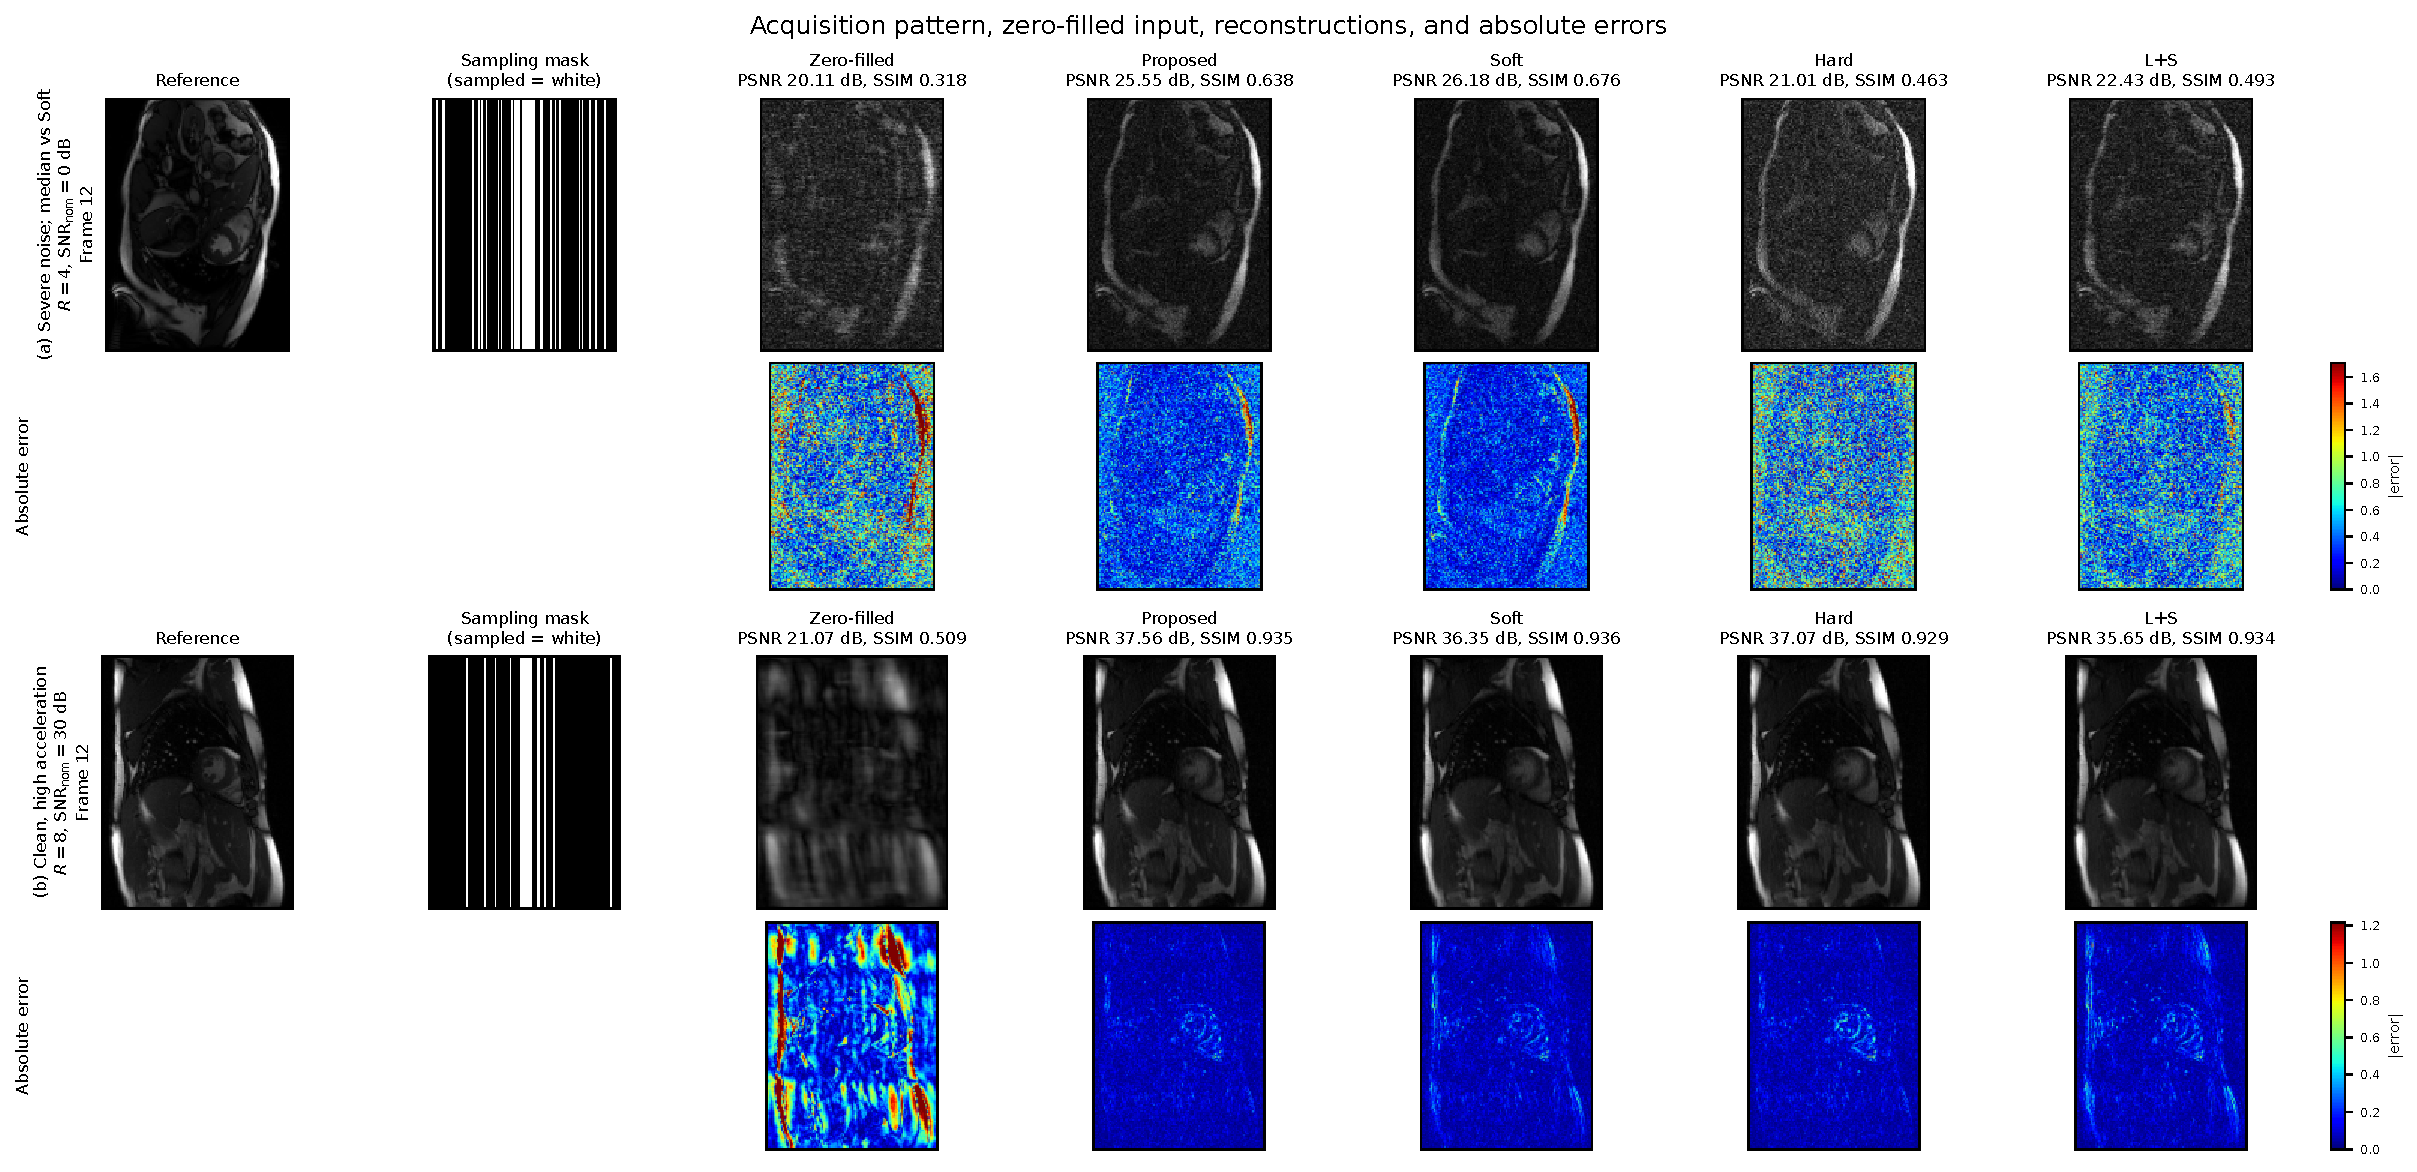
\includegraphics[width=\textwidth]{fig6_qualitative_temporal_comparison.pdf}
  \caption{Reference images, sampling masks (white denotes acquired phase-encoding locations), noisy zero-filled inputs, reconstructions, and magnitude absolute-error maps. (a) $R=4$, $\mathrm{SNR}_{\mathrm{nom}}=0$~dB; (b) $R=8$, $\mathrm{SNR}_{\mathrm{nom}}=30$~dB. The middle cardiac frame is displayed; PSNR and SSIM were calculated over the complete cine.}
  \label{fig:qualitative_temporal}
\end{figure*}

\subsection{Protocol diagnostics}
\label{sec:protocol_diagnostics}

\subsubsection{Pilot-only parameter-boundary audit}
\label{sec:boundary_audit}

Candidate ranges were expanded only when a pilot-series validation winner lay on a lower or upper boundary and its improvement over the adjacent interior candidate exceeded the numerical tolerance. The corresponding coordinate was moved outward while the remaining coordinates were held fixed, and the new candidates were evaluated with unchanged masks, noise, validation splits, and stopping rules. Six rounds evaluated 97 outward settings, corresponding to 388 pilot reconstructions, with no failures; the sixth round produced no further trigger. The candidate sets were then frozen before formal evaluation. No boundary-driven search was performed on the 20 formal series, because doing so would adapt the tuning space to the evaluation data. Additional boundary experiments are unnecessary under the frozen 300-iteration protocol, but the audit must be repeated if the stopping rule or selection protocol changes.

\subsubsection{Convergence and iteration-cap sensitivity}
\label{sec:convergence_sensitivity}

The relative tolerance was reached within 300 iterations in 74/240 Proposed, 175/240 Soft, 238/240 Hard, and 40/240 L+S formal refits; otherwise the run ended at the common cap. The primary comparison is therefore between prespecified early-stopped procedures.

With selected parameters held fixed, representative runs were continued to 600 iterations. For Proposed and L+S in the four corner conditions $R\in\{4,8\}$ and $\mathrm{SNR}_{\mathrm{nom}}\in\{0,30\}$~dB, all eight runs reached tolerance by 600 iterations, the largest absolute PSNR change was 0.104~dB, and no Proposed--L+S ordering changed. In the targeted $R=4$, 10-dB Proposed--Hard case, the gap changed from $-0.139$ to $-0.855$~dB because Proposed decreased by 0.716~dB while Hard remained unchanged after converging at iteration 140. The isolated formal reversal is therefore not explained by an iteration cap that favoured Hard. Because changing the cap alters the coupled tuning-and-stopping procedure, 300 iterations was retained for the primary experiment; a 600-iteration primary protocol would require renewed pilot tuning and boundary auditing.

\begin{figure*}[t]
  \centering
  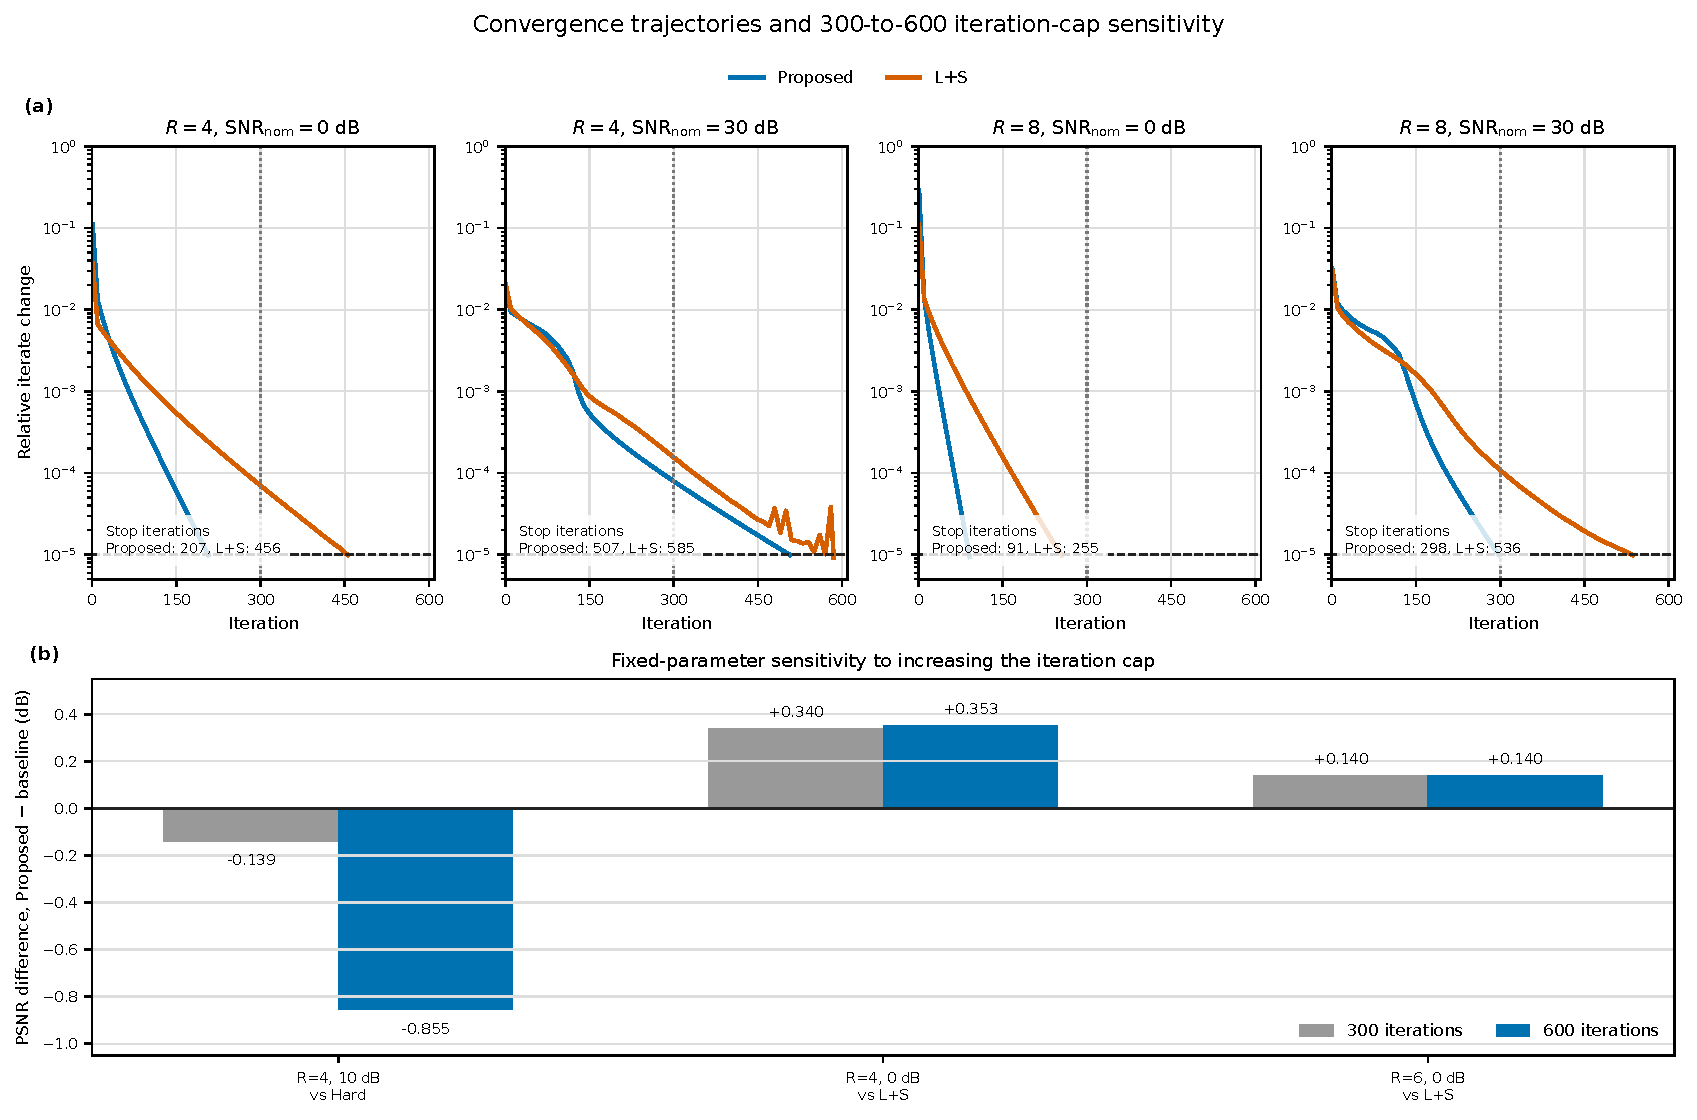
\includegraphics[width=\textwidth]{fig3_convergence_sensitivity.pdf}
  \caption{Convergence and iteration-cap sensitivity. Relative iterate changes are shown for representative Proposed and L+S corner conditions, together with Proposed-minus-baseline PSNR differences at 300 and 600 iterations for targeted comparisons. Parameters were held fixed during continuation.}
  \label{fig:convergence_sensitivity}
\end{figure*}

\subsection{Discussion and limitations}
\label{sec:evaluation_discussion}

The proposed rule was generally preferable to Hard thresholding and showed a condition-dependent trade-off relative to Soft and L+S. Conventional stronger shrinkage was often more stable at 0--10~dB, whereas Proposed became competitive at 20~dB and was favourable in PSNR at all 30-dB conditions. This pattern is consistent with reduced shrinkage bias in dominant temporal components when measurement noise is small, but the experiment does not isolate that mechanism causally. The non-monotone 0-dB results are plausible because, by construction, the acquired-signal and added-noise RMS values are equal; anatomy, sampling, and validation selection then produce broad and skewed paired differences.

The study contains 20 OCMR series, and patient-level independence could not be confirmed. Undersampling and Gaussian noise were retrospective, and ESPIRiT maps and references were derived from fully sampled data before degradation. Coil combination also limits the conclusions to the stated single-image protocol rather than a sensitivity-encoded multi-coil reconstruction. Candidate sets were constructed from four pilot series, and the convergence analysis used representative cases rather than the complete cohort. Finally, image-fidelity metrics were not linked to a blinded reader or clinical task. Within these limits, the evidence supports a robust advantage over Hard in most conditions and a noise-dependent, rather than universal, advantage over Soft and L+S.
